\documentclass{ctexart}
\usepackage{listings}
\usepackage{amsmath}
\usepackage{amssymb}
\usepackage{setspace}
\usepackage{enumitem}
\usepackage{changepage}
\usepackage{graphicx,caption}
\usepackage{listings}
\usepackage{color}
\lstset{       
	numbers=left,                                        % 在左侧显示行号
	frame = leftline,
	numberstyle=\tiny\color{gray},                       % 设定行号格式             
	backgroundcolor=\color[RGB]{245,245,244},            % 设定背景颜色
	keywordstyle=\color[RGB]{40,40,255},                 % 设定关键字颜色
	numberstyle=\footnotesize\color{blue},           
	commentstyle=\it\color[RGB]{0,96,96},                % 设置代码注释的格式
	stringstyle=\rmfamily\slshape\color[RGB]{128,0,0},   % 设置字符串格式
	showstringspaces=false,                              % 不显示字符串中的空格
	language=c++,                                        % 设置语言
}
\title{\Huge 词法分析设计文档}
\author{18373054 陆晓东}
\begin{document}
	\maketitle
	\newpage
	\section{编码前设计}
	\subsection{识别单词划分}
	对于需要识别的单词,可以根据单词的特性进行划分。这里主要按照树状结构进行了划分。然后对于不同划分层次的单词进行不同
	的识操作和处理操作。\par
	首先可以将只需读入一个字符就能判定类别的单字符分为一类,叫做单符号判定类。其他类别叫做多符号判断类。在多符号判断类中,first集合独一无二且长度固定的类别叫做直接可判断类(!=等)。first有重复且长度固定的称为前缀相同类。长度不固定的为循环读入类。循环读入类有字符常量,字符串,标识符\&保留字类。
	\begin{figure}[htbp]
		\centering
		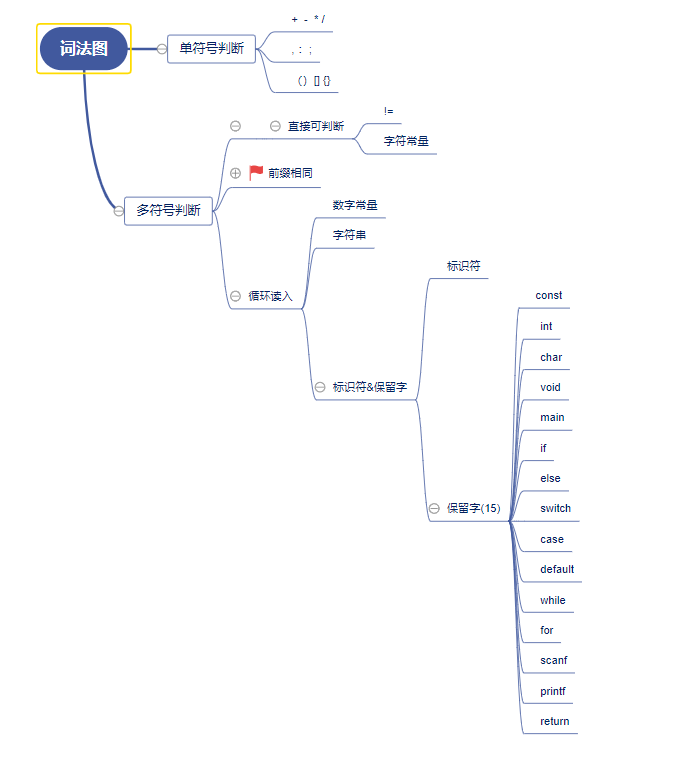
\includegraphics[width=0.5\linewidth]{pics/cf.PNG}
		\caption{分类示意图} \label{figs:cf}
	\end{figure}
	\subsection{编码方案}
	根据不同分类采取不同的处理方案
	\begin{enumerate}
		\item 单字符可以分隔:直接读入即可
		\item 直接可判定类:
		\begin{enumerate}
			\item != : 再读入一个字符即可,若不是$=$则直进入错误处理,否则转出
			\item 字符常量:读入两个字符c1,c2,若c2不为'或者c1不为字符常量,则进入错误处理,否则转出
		\end{enumerate}
		\item 前缀相同: 再读入一个字符,若为$=$则当作前缀相同中长的处理,否则当作短的处理并且退回一个单词
		\item 循环读入类 
		\begin{enumerate}
			\item 数字常量:重复读入知道不为$0-9$ 之间的单词,最后吐出一个
			\item 字符串:重复读入直到不合法字符串组成元素,若最后读到字符不为"则进入错误处理,否则退出
			\item 标识符\&保留字:重复读入直到不为数字或者字符,退回最后读入的一个。和保留字一一比较,若有相同的则当保留字
			处理,否则当标识符处理
		\end{enumerate}
	\end{enumerate}
\newpage
\section{编码完成后修改}
编码完成后主要对读入eof后退回字符可能导致多次读入的情况,增加了对eof的处理。(主要针对不符合文法情况的代码)
\begin{lstlisting}[caption=修改后核心代码]
	 int c=0;
	string ms;
	while(true){
	ms.clear();
	c = fgetc(fp);
	while(c==' '||c=='\n'||c=='\t'||c=='\r'){
	c = fgetc(fp);
	}
	if(c==-1) break;
	//@signle
	if(c=='('){
	ms.push_back(c);
	add(LPARENT,ms);
	}else if(c==')'){
	ms.push_back(c);
	add(RPARENT,ms);
	}else if(c=='['){
	ms.push_back('[');
	add(LBRACK,ms);
	}else if(c==']'){
	ms.push_back(']');
	add(RBRACK,ms);
	}
	else if(c=='{'){
	ms.push_back(c);
	add(LBRACE,ms);
	}else if(c=='}'){
	ms.push_back(c);
	add(RBRACE,ms);
	}else if(c=='+'){
	ms.push_back(c);
	add(PLUS,ms);
	}else if(c=='-'){
	ms.push_back(c);
	add(MINU,ms);
	}else if(c=='*'){
	ms.push_back(c);
	add(MULT,ms);
	}else if(c=='/'){
	ms.push_back(c);
	add(DIV,ms);
	}else if(c==','){
	ms.push_back(c);
	add(COMMA,ms);
	}else if(c==':'){
	ms.push_back(c);
	add(COLON,ms);
	}else if(c==';'){
	ms.push_back(c);
	add(SEMICN,ms);
	}
	//@doubel+
	else if(c=='!'){
	c = fgetc(fp);
	if(c!='=') error(0);
	else{
	ms.append("!=");
	add(NEQ,ms);
	}
	}
	else if(c=='='){ // ==\=
	ms.push_back(c);
	c = fgetc(fp);
	if(c=='='){
	ms.push_back(c);
	add(EQL,ms);
	}else{
	fseek(fp,-1,SEEK_CUR);
	add(ASSIGN,ms);
	}
	}
	else if(c=='<'){ //<\<=
	ms.push_back(c);
	c = fgetc(fp);
	if(c=='='){
	ms.push_back(c);
	add(LEQ,ms);
	}else{
	fseek(fp,-1,SEEK_CUR);
	add(LSS,ms);
	}
	}
	else if(c=='>'){ // >\>= 
	ms.push_back(c);
	c = fgetc(fp);
	if(c=='='){
	ms.push_back(c);
	add(GEQ,ms);
	}else{
	fseek(fp,-1,SEEK_CUR);
	add(GRE,ms);
	}
	}
	else if(c=='\"'){
	c = fgetc(fp);
	while(ISSTR(c)){
	ms.push_back(c);
	c = fgetc(fp);
	}
	
	if(c!='\"') error(0);
	else add(STRCON,ms);
	
	}else if(c=='\''){
	char mc1=fgetc(fp),mc2=fgetc(fp);
	if(mc2!='\''||!ISCHAR(mc1)){
	error(0);
	}else{
	ms.push_back(mc1);
	add(CHARCON,ms);
	}
	}
	//@multi
	else if(ISDIGIT(c)){ 
	ms.push_back(c);
	c= fgetc(fp);
	while(ISDIGIT(c)){
	ms.push_back(c);
	c = fgetc(fp);
	}
	fseek(fp,-1,SEEK_CUR);
	add(INTCON,ms);
	}
	else if(ISALPHA(c)){ //15 special && 1 common
	ms.push_back(c);
	c = fgetc(fp);
	while(ISALPHA(c)||ISDIGIT(c)){
	ms.push_back(c);
	c= fgetc(fp);
	}
	string mms = ms;
	for(auto it=mms.begin();it!=mms.end();it++){
	*it = LOWER((*it));
	}
	if(mms.compare("const")==0){
	add(CONSTTK,ms);
	}else if(mms.compare("int")==0){
	add(INTTK,ms);
	}else if(mms.compare("char")==0){
	add(CHARTK,ms);
	}else if(mms.compare("void")==0){
	add(VOIDTK,ms);
	}else if(mms.compare("main")==0){
	add(MAINTK,ms);
	}else if(mms.compare("if")==0){
	add(IFTK,ms);
	}else if(mms.compare("else")==0){
	add(ELSETK,ms);
	}else if(mms.compare("switch")==0){
	add(SWITCHTK,ms);
	}else if(mms.compare("case")==0){
	add(CASETK,ms);
	}else if(mms.compare("default")==0){
	add(DEFAULTTK,ms);
	}else if(mms.compare("while")==0){
	add(WHILETK,ms);
	}else if(mms.compare("for")==0){
	add(FORTK,ms);
	}else if(mms.compare("scanf")==0){
	add(SCANFTK,ms);
	}else if(mms.compare("printf")==0){
	add(PRINTFTK,ms);
	}else if(mms.compare("return")==0){
	add(RETURNTK,ms);
	}
	else{
	add(IDENFR,ms);
	}
	if(c!=-1) fseek(fp,-1,SEEK_CUR); //eof pd
	}else{
	error(0);
	}
	
	}
\end{lstlisting}
\end{document}